\subsubsection{Análisis de casos}
\subsubsubsection{Iteraciones}
\paragraph{}
Lo primero a tener en cuenta para el análisis de esta heurística es profundizar lo que sucede en cada iteración del ciclo. Como mencionamos al analizar la complejidad tuvimos en cuenta los tipos de instancias sobre las que experimentaríamos para no tener problemas al poner una cota sobre la cantidad de iteraciones. Esto fue necesario ya que de otra forma no tendríamos un aproximado sobre lo que puede tardar nuestro algoritmo: y aún así, como veremos en la experimentación, el tiempo de ejecución de kmeans dependerá de muchos factores.
\paragraph{}
En general, podemos notar que para las instancias utilizadas se realizan pocas iteraciones. En el siguiente ejemplo, vemos como se van modificando los centroids representados por una cruz (\textbf{+}) a medida que va cambiando la pertenencia de los puntos a distintos clusters. En este caso particular, los centroids iniciales se encuentran dispersos en el plano. Observamos que el mayor cambio de ubicación y pertenencia se da entre las primeras iteraciones: a medida que avanza el procedimiento los centroids se mueven menos y pocos puntos cambian de color (es decir, de cluster o más bien de ruta). Eso indicaría ya con unas pocas iteraciones de kmeans se puede llegar a una solución bastante aproximada del problema. 
\paragraph{}
Un dato no menor del estado en cada paso es que la cantidad de clusters desde el principio hasta el final se mantiene constante. En los siguientes puntos entraremos en más detalle acerca de esto.
\begin{figure}[H]
	\centering
	\begin{minipage}[t]{.3\textwidth}
		\centering
		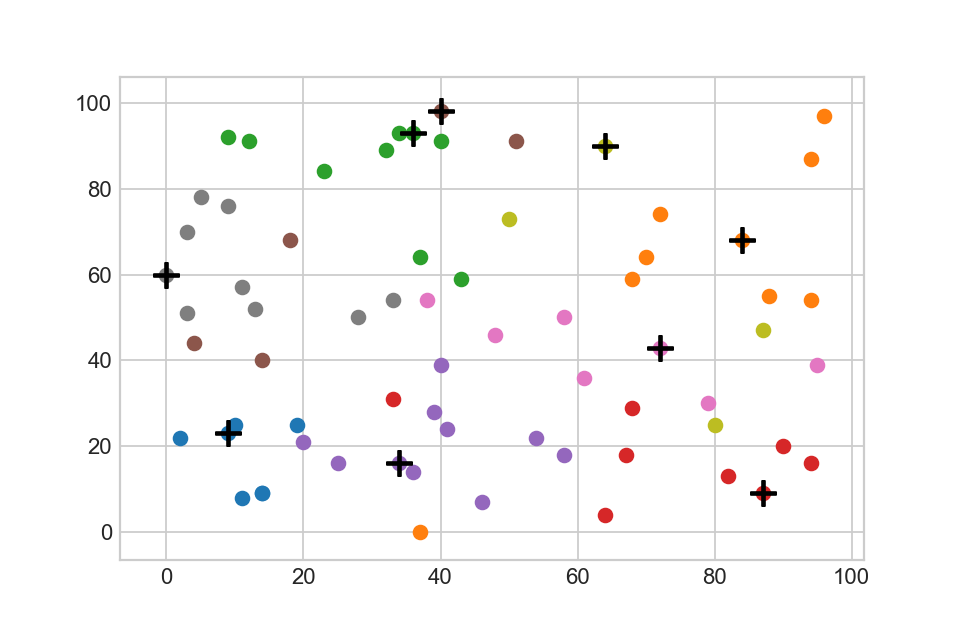
\includegraphics[scale=0.4]{kmeans/A-n69-cluster0}
	\end{minipage}\qquad
	\begin{minipage}[t]{.3\textwidth}
		\centering
		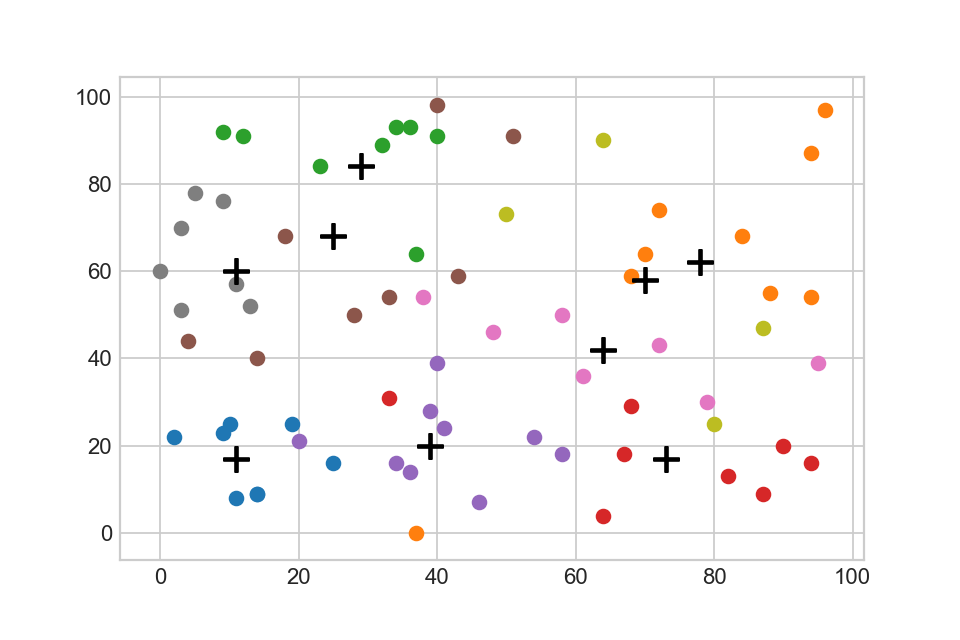
\includegraphics[scale=0.4]{kmeans/A-n69-cluster1}
	\end{minipage}\qquad
	\begin{minipage}[t]{.3\textwidth}
		\centering
		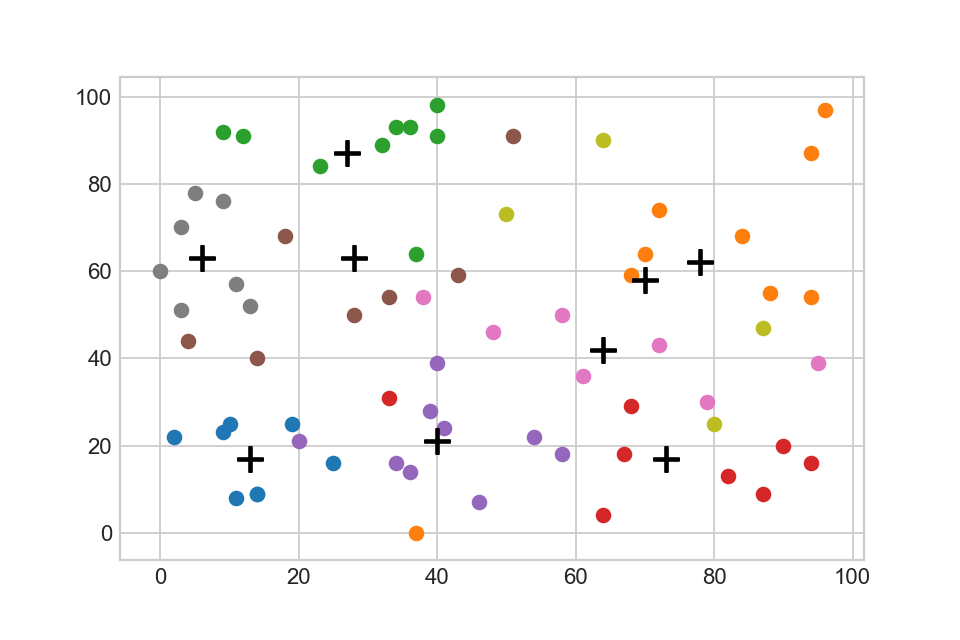
\includegraphics[scale=0.4]{kmeans/A-n69-cluster2}
	\end{minipage}\qquad
	\begin{minipage}[t]{.3\textwidth}
		\centering
		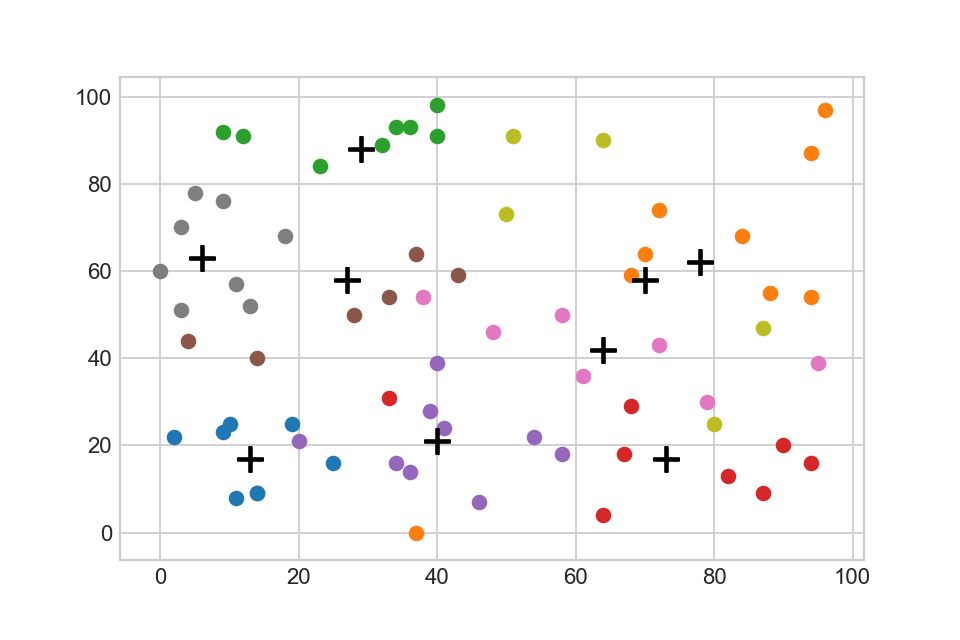
\includegraphics[scale=0.4]{kmeans/A-n69-cluster3}
	\end{minipage}\qquad
	\begin{minipage}[t]{.3\textwidth}
		\centering
		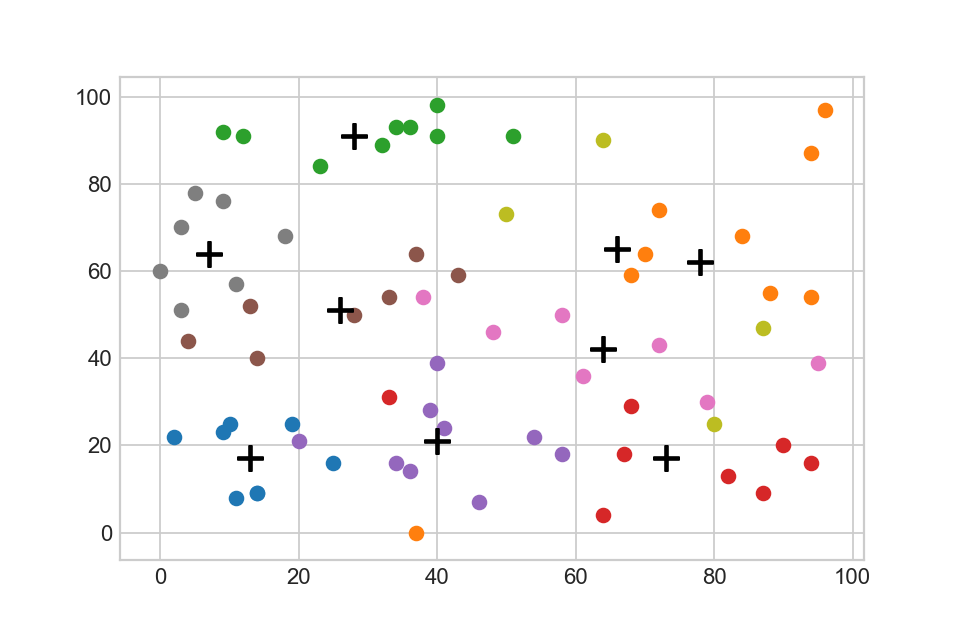
\includegraphics[scale=0.4]{kmeans/A-n69-cluster4}
	\end{minipage}\qquad
	
	Estado luego de asignar nodos a clusters, cinco iteraciones en total.
\end{figure}

\subsubsubsection{Centroids iniciales}
\paragraph{}
Kmeans tiene ciertas limitaciones. Un ejemplo claro es que al elegir los nodos random o, en nuestro caso, los primeros de la entrada, el orden en el que entran los datos puede afectar la performance del algoritmo (a diferencia de savings por ejemplo). 
\paragraph{}
Para que el resultado se vea efectivamente perturbado por esta elección inicial, mostraremos un caso particular y como resulta para cada entrada. Pensemos que sucede si luego de la primera iteración, al intentar cambiar de cluster a cada punto la demanda de estos es mayor que la capacidad restante del camión: en este tipo de instancias, habrá menos posibilidad de que se den cambios de cluster. Presentemos una analogía a esta situación: un estado de tetris cuando al no encajar perfectamente piezas quedan espacios imposibles de rellenar. 

\begin{figure}[H]
	\centering
	\begin{minipage}{0.35\textwidth}
		\centering
		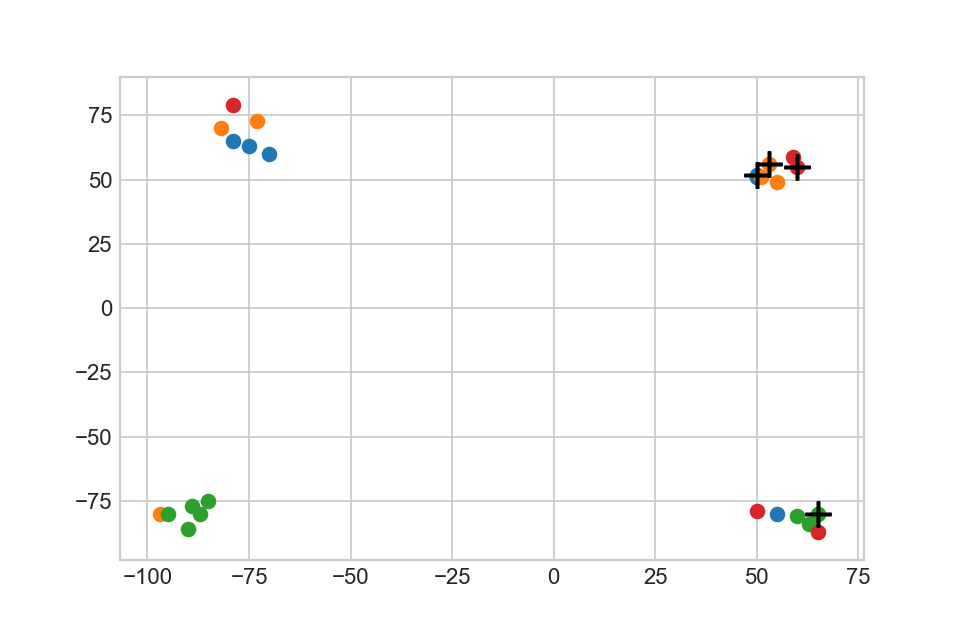
\includegraphics[width=1\textwidth]{images/kmeans/malonube0}
		%\caption{\footnotesize Clusters iniciales}
		%\label{fig:kmeans-malo-grande}
	\end{minipage}%
	\hspace{0.03\textwidth}
	\begin{minipage}{0.35\textwidth}
		\centering
		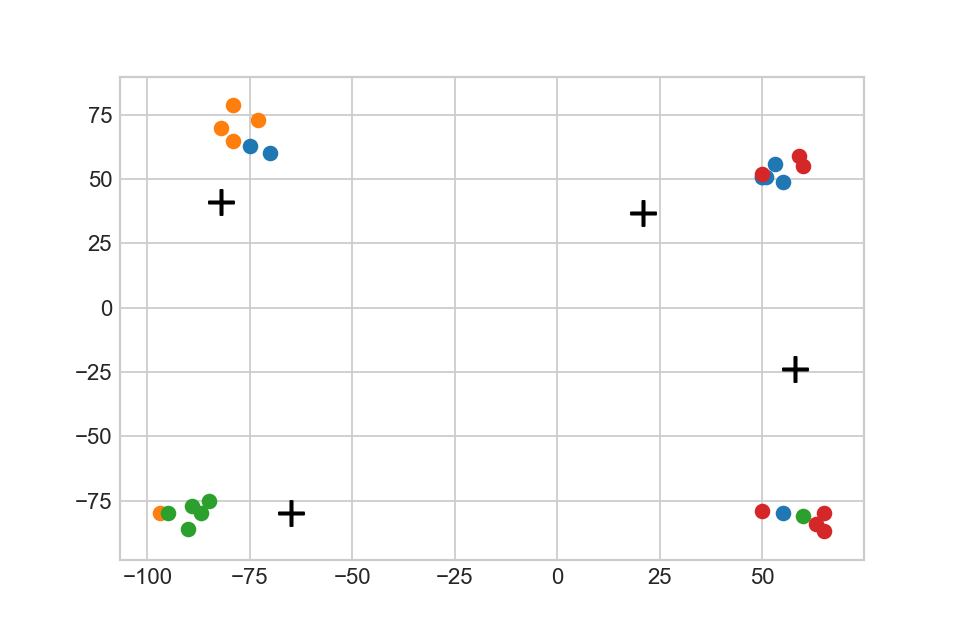
\includegraphics[width=1\textwidth]{images/kmeans/malonubefin}
		%\caption{\footnotesize Clusters iniciales con otra elección de primeros nodos}
		%\label{fig:savings-optimo-granxxde}
	\end{minipage}%
\end{figure}
\begin{figure}[H]
	\centering
	\begin{minipage}{0.35\textwidth}
		\centering
		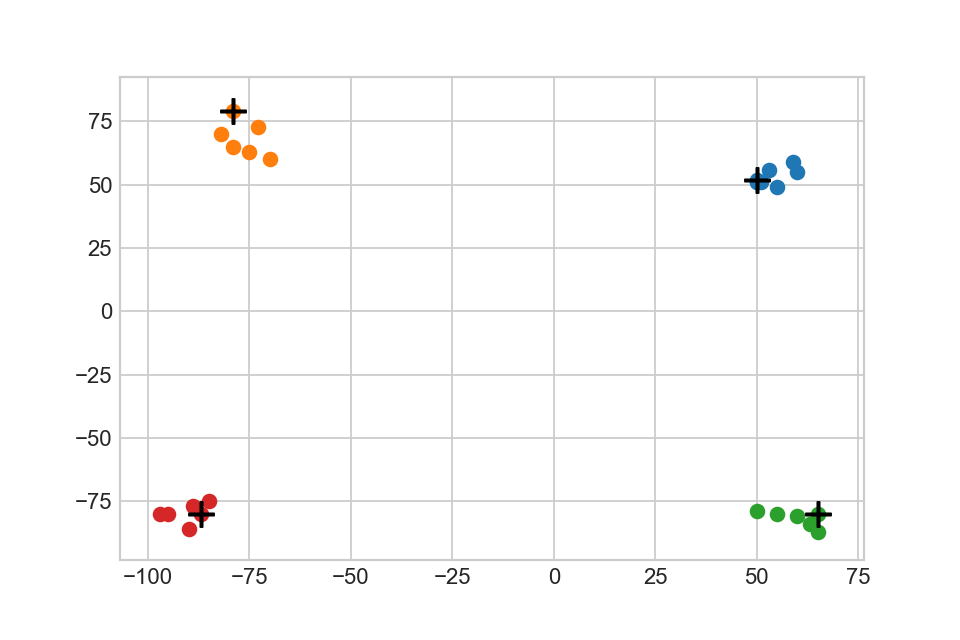
\includegraphics[width=1\textwidth]{images/kmeans/buenonube0}
		%\caption{\footnotesize Clusters iniciales}
		%\label{fig:kmeans-malo-gramnde}
	\end{minipage}%
	\hspace{0.03\textwidth}
	\begin{minipage}{0.35\textwidth}
		\centering
		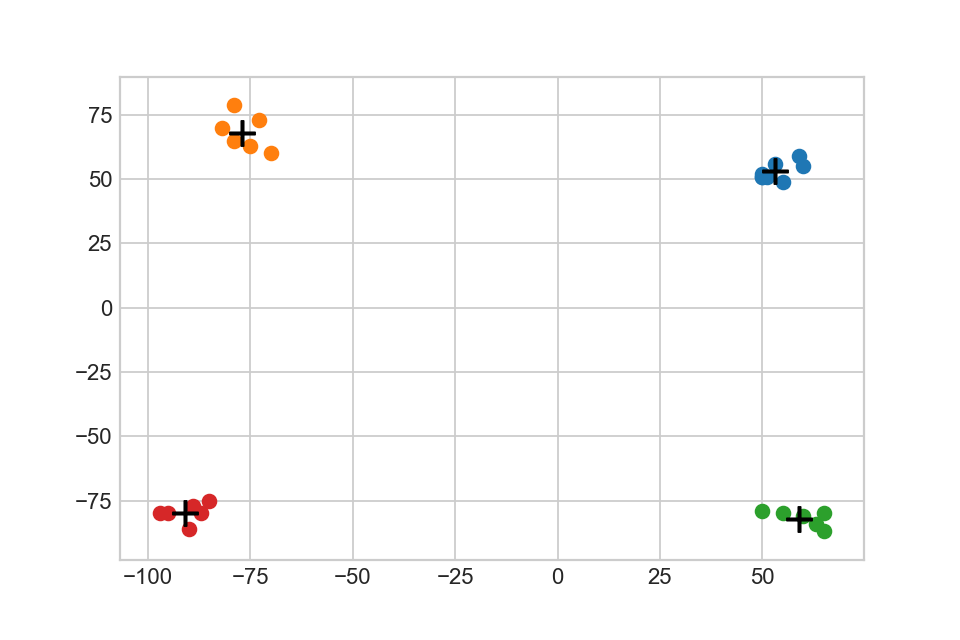
\includegraphics[width=1\textwidth]{images/kmeans/buenonube2}
		%\caption{\footnotesize Clusters iniciales con otra elección de primeros nodos}
		%\label{fig:savings-optimo-gkranxxde}
	\end{minipage}%
\end{figure}
\paragraph{}
En el primer par de figuras mostramos este caso de mala elección de nodos que llevará a una mala solución final. Como podemos observar, la asignación de clusters cambia muy poco de principio a fin. El otro par de figuras corresponde a una entrada que favorece la performance del algoritmo. Es un caso claro de grafo de tipo ``nubes'' donde si elegimos un centroid en cada una de ellas y es posible en términos de capacidad suplir a todos los clientes de esa ruta, se puede llegar a una solución cercana a la óptima.

\begin{figure}[H]
	\centering
	\begin{minipage}{0.38\textwidth}
		\centering
		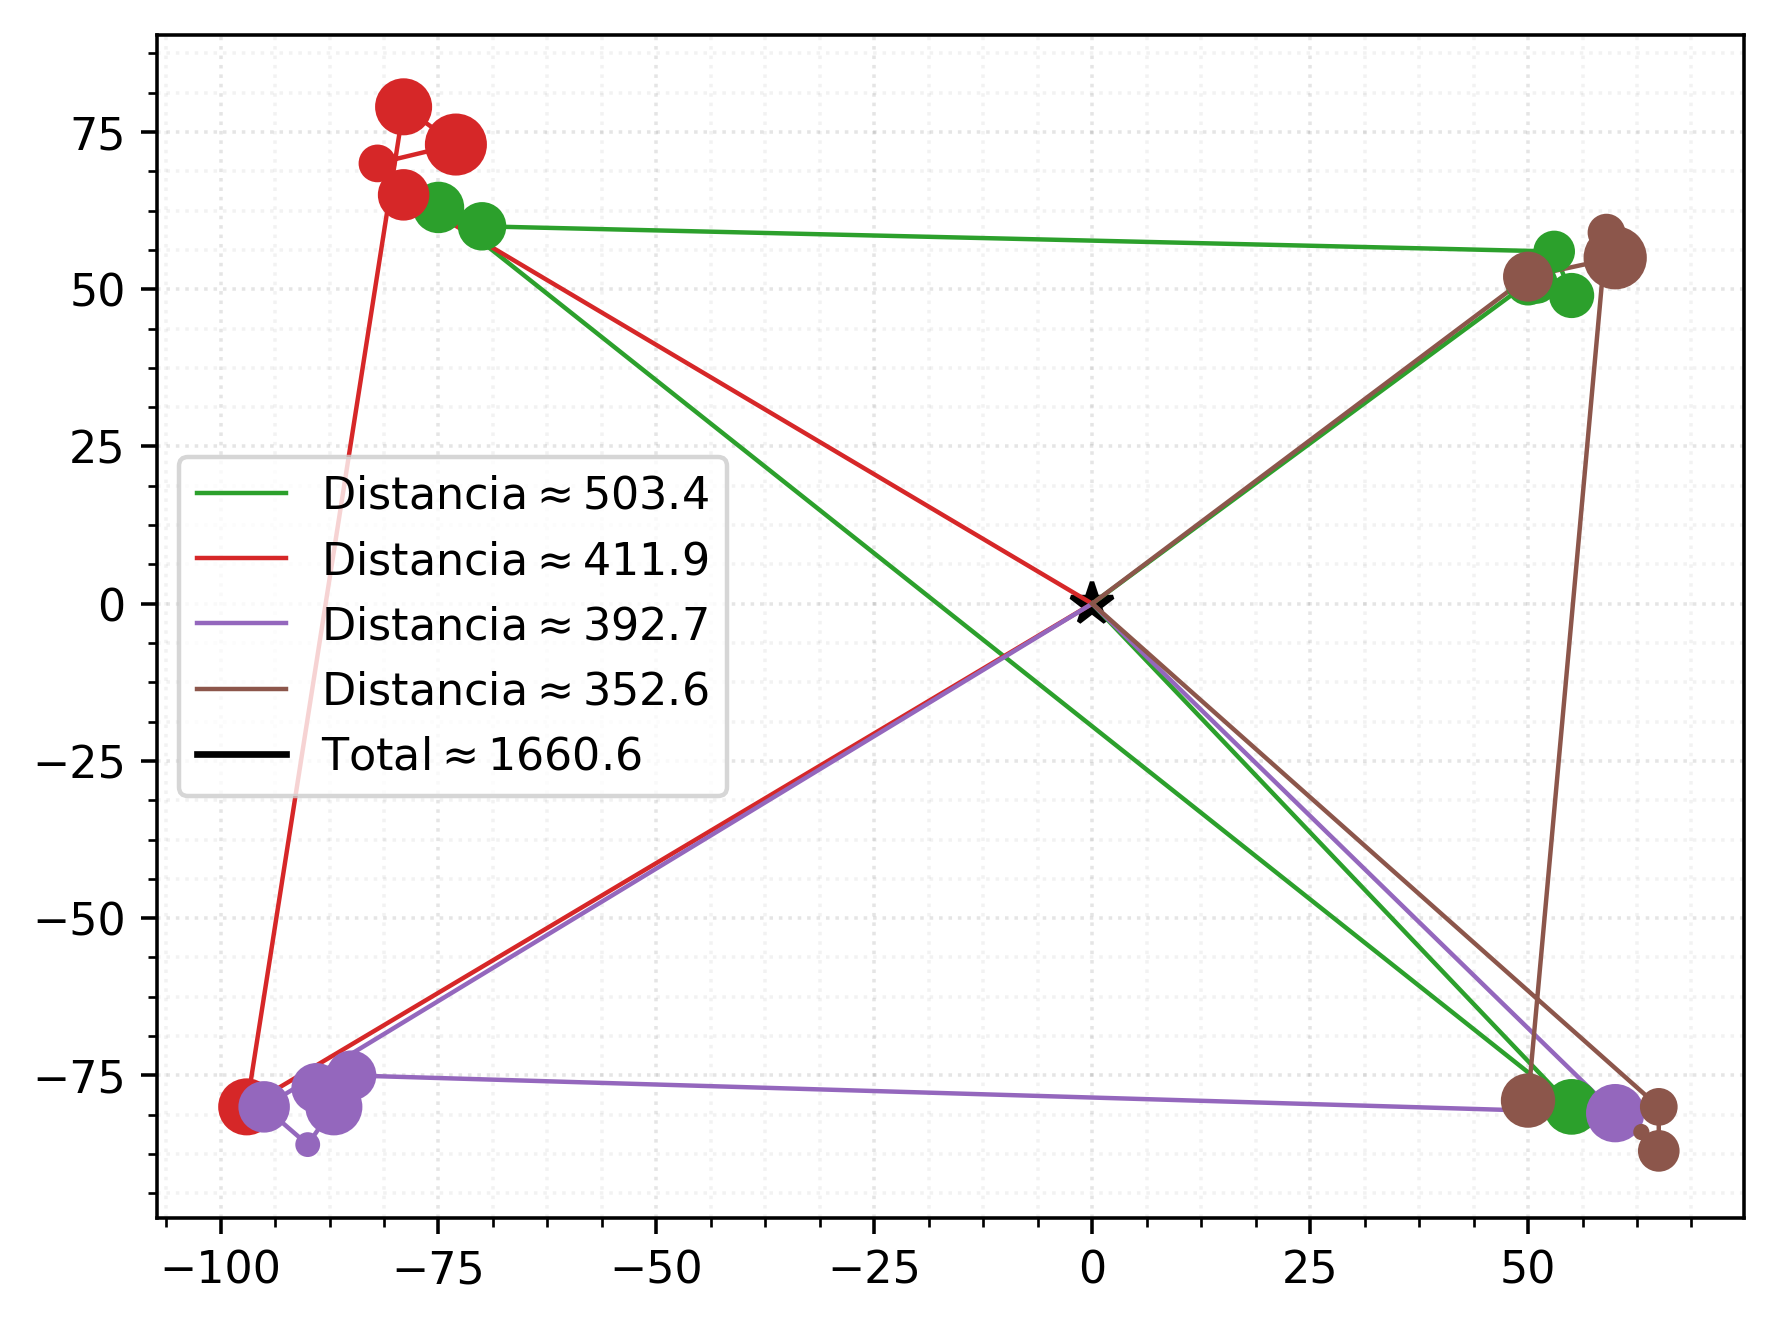
\includegraphics[width=1\textwidth]{images/kmeans/nubemalodistancia}
		\caption{\footnotesize Solución con centroids iniciales desfavorables}
		\label{fig:kmeans-mala-entrada}
	\end{minipage}%
	\hspace{0.03\textwidth}
	\begin{minipage}{0.38\textwidth}
		\centering
		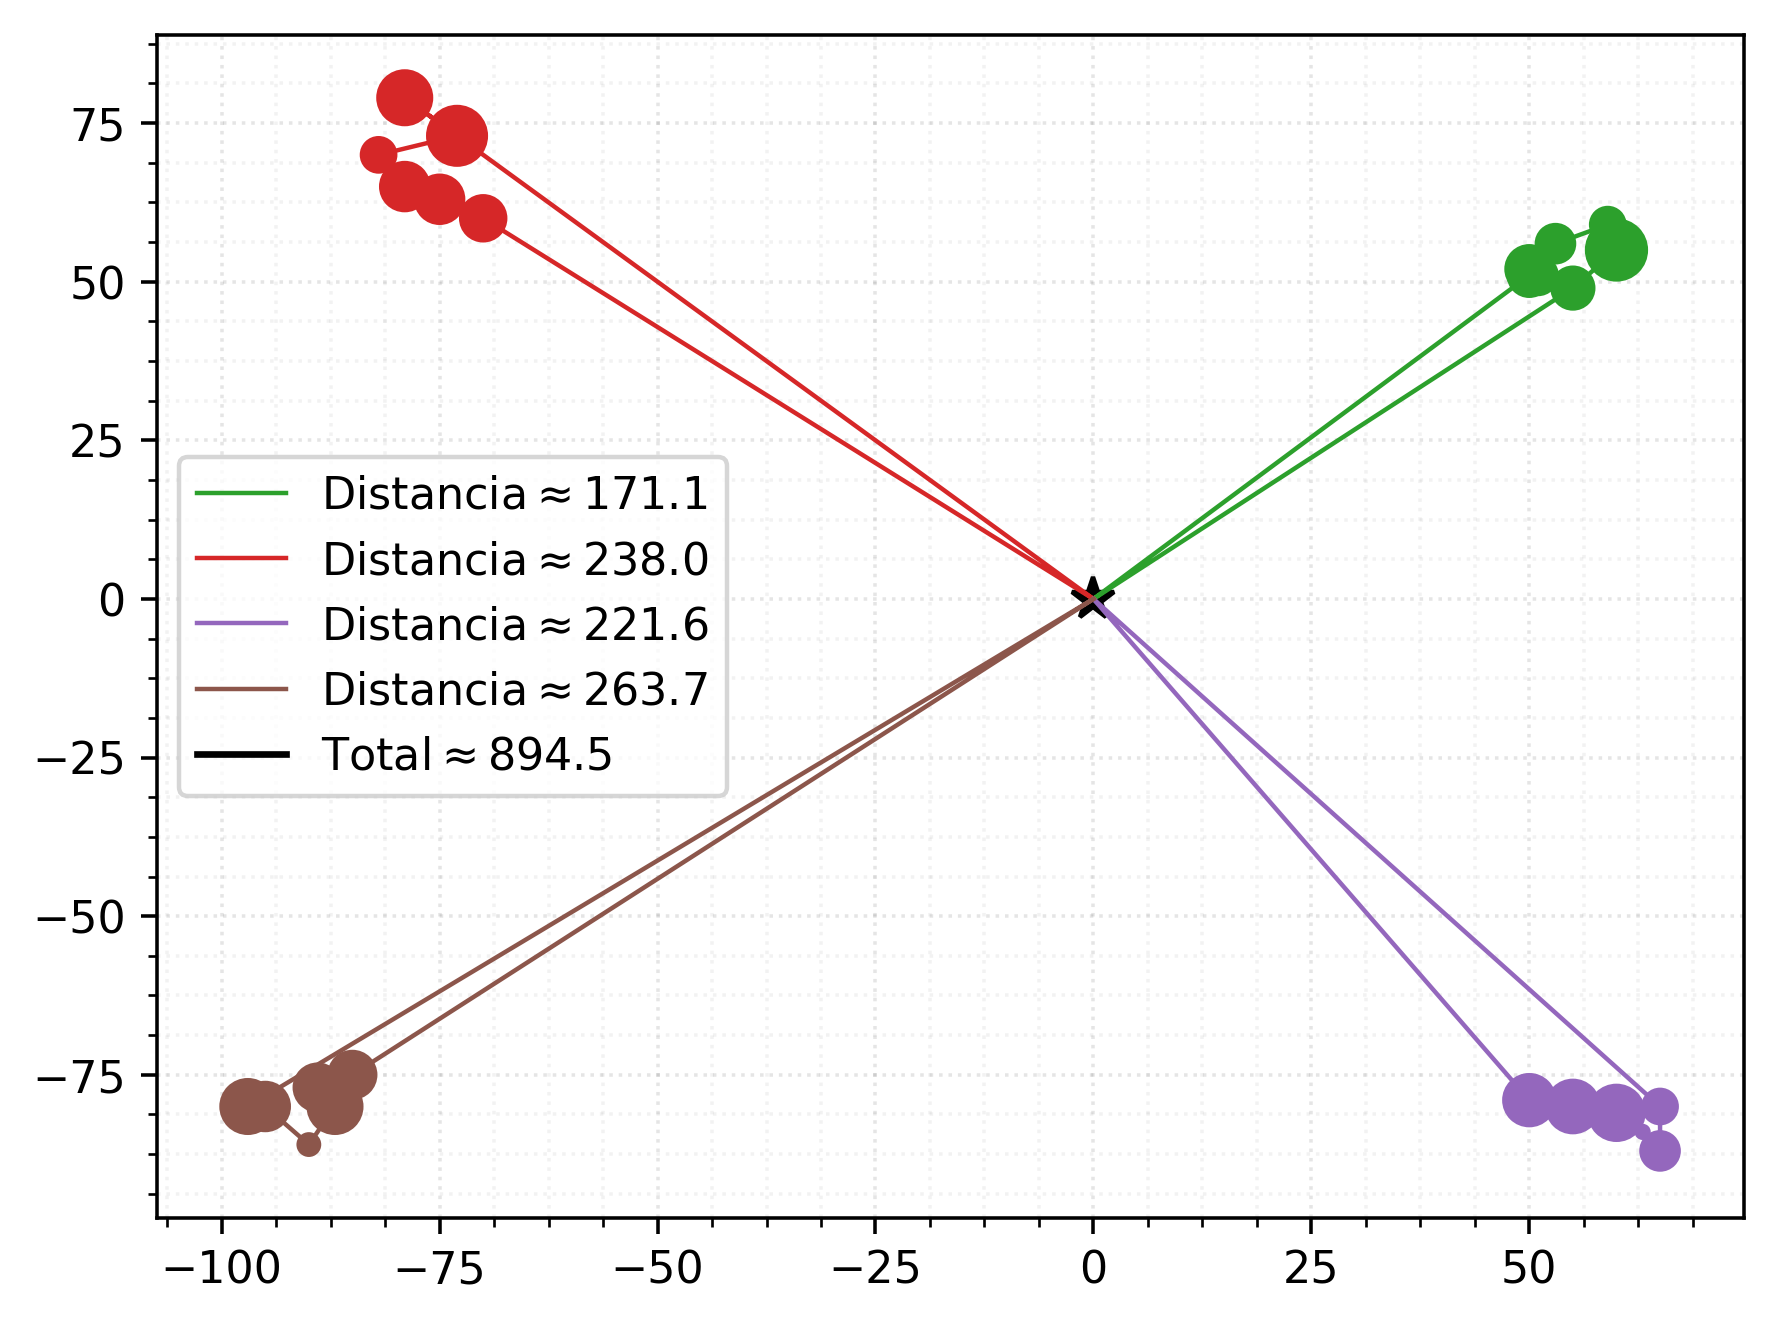
\includegraphics[width=1\textwidth]{images/kmeans/nubebuenodistancia}
		\caption{\footnotesize Solución con centroids iniciales favorables}
		\label{fig:kmeans-buena-entrada}
	\end{minipage}%
\end{figure}
\paragraph{}
En la figura \ref{fig:kmeans-mala-entrada} tenemos la solución desfavorable, que comparada con la que da savings (en este caso, mejor que la favorable de kmeans da 883 aproximadamente), es 88\% peor. Por otro lado, el caso favorable de la figura \ref{fig:kmeans-buena-entrada} está muy cerca de la que da savings, como era de esperarse, siendo sólamente un 1.3\% peor.



